\section{Our Approach}
\label{sec:algo}
In this section, we introduce our approach to solve the problem.

%\subsection{Preliminaries}
Before the discussion, we will use some terms as defined below:

{\bf Target Number K:}

{\bf DOM Tree:} 	
%A DOM Tree is blabla....

{\bf Node:}		
By default, a node means a DOM Tree node in this paper.
There are three main kinds of nodes, which are tag nodes, text nodes and remark nodes.

{\bf Tag:}		
A tag is one kind of node, which may has some attributes and can contain children nodes.
%blabla

{\bf Web Page:}
Since nowadays web pages are mostly presented in HTML, it is common to use DOM Tree Structure to represent and analyse those pages.
Therefore in this paper, we would like to use a DOM Tree, or the root node of the tree to represent a web page.

{\bf Data Record:}
A data record is a HTML segment in top-$k$ pages which represent an item in top-$k$ list.
As a component of the web page, a data record can be represented by a subtree (or a child node) of the entire DOM tree.

{\bf Data Record Component:}
As its literal meaning,
a Data Record Component is a component of a data record, which can be a title, a text description or a picture of the data record.
As a component of the data record, a data record component can be represented by a subtree (or a child node) of data record.

{\bf Data Record Title:}
A data record title is a data record component, which is usually in the form of short brief text.
A title gives the name of the data record, which is the key infomation of a list item.

{\bf Data Record List:}
There should be $k$ data records in a top-$k$ page, those data records can form a data record list.
According to the definition of data record, a data record list can be represented by a DOM node list.

%Data Record Tree(DRT):
%Data Record Tree List(DRT List):
{\bf Tag Path:}

{\bf Visual Region Area(VRA):}

\begin{figure*}[th]
	\centering
	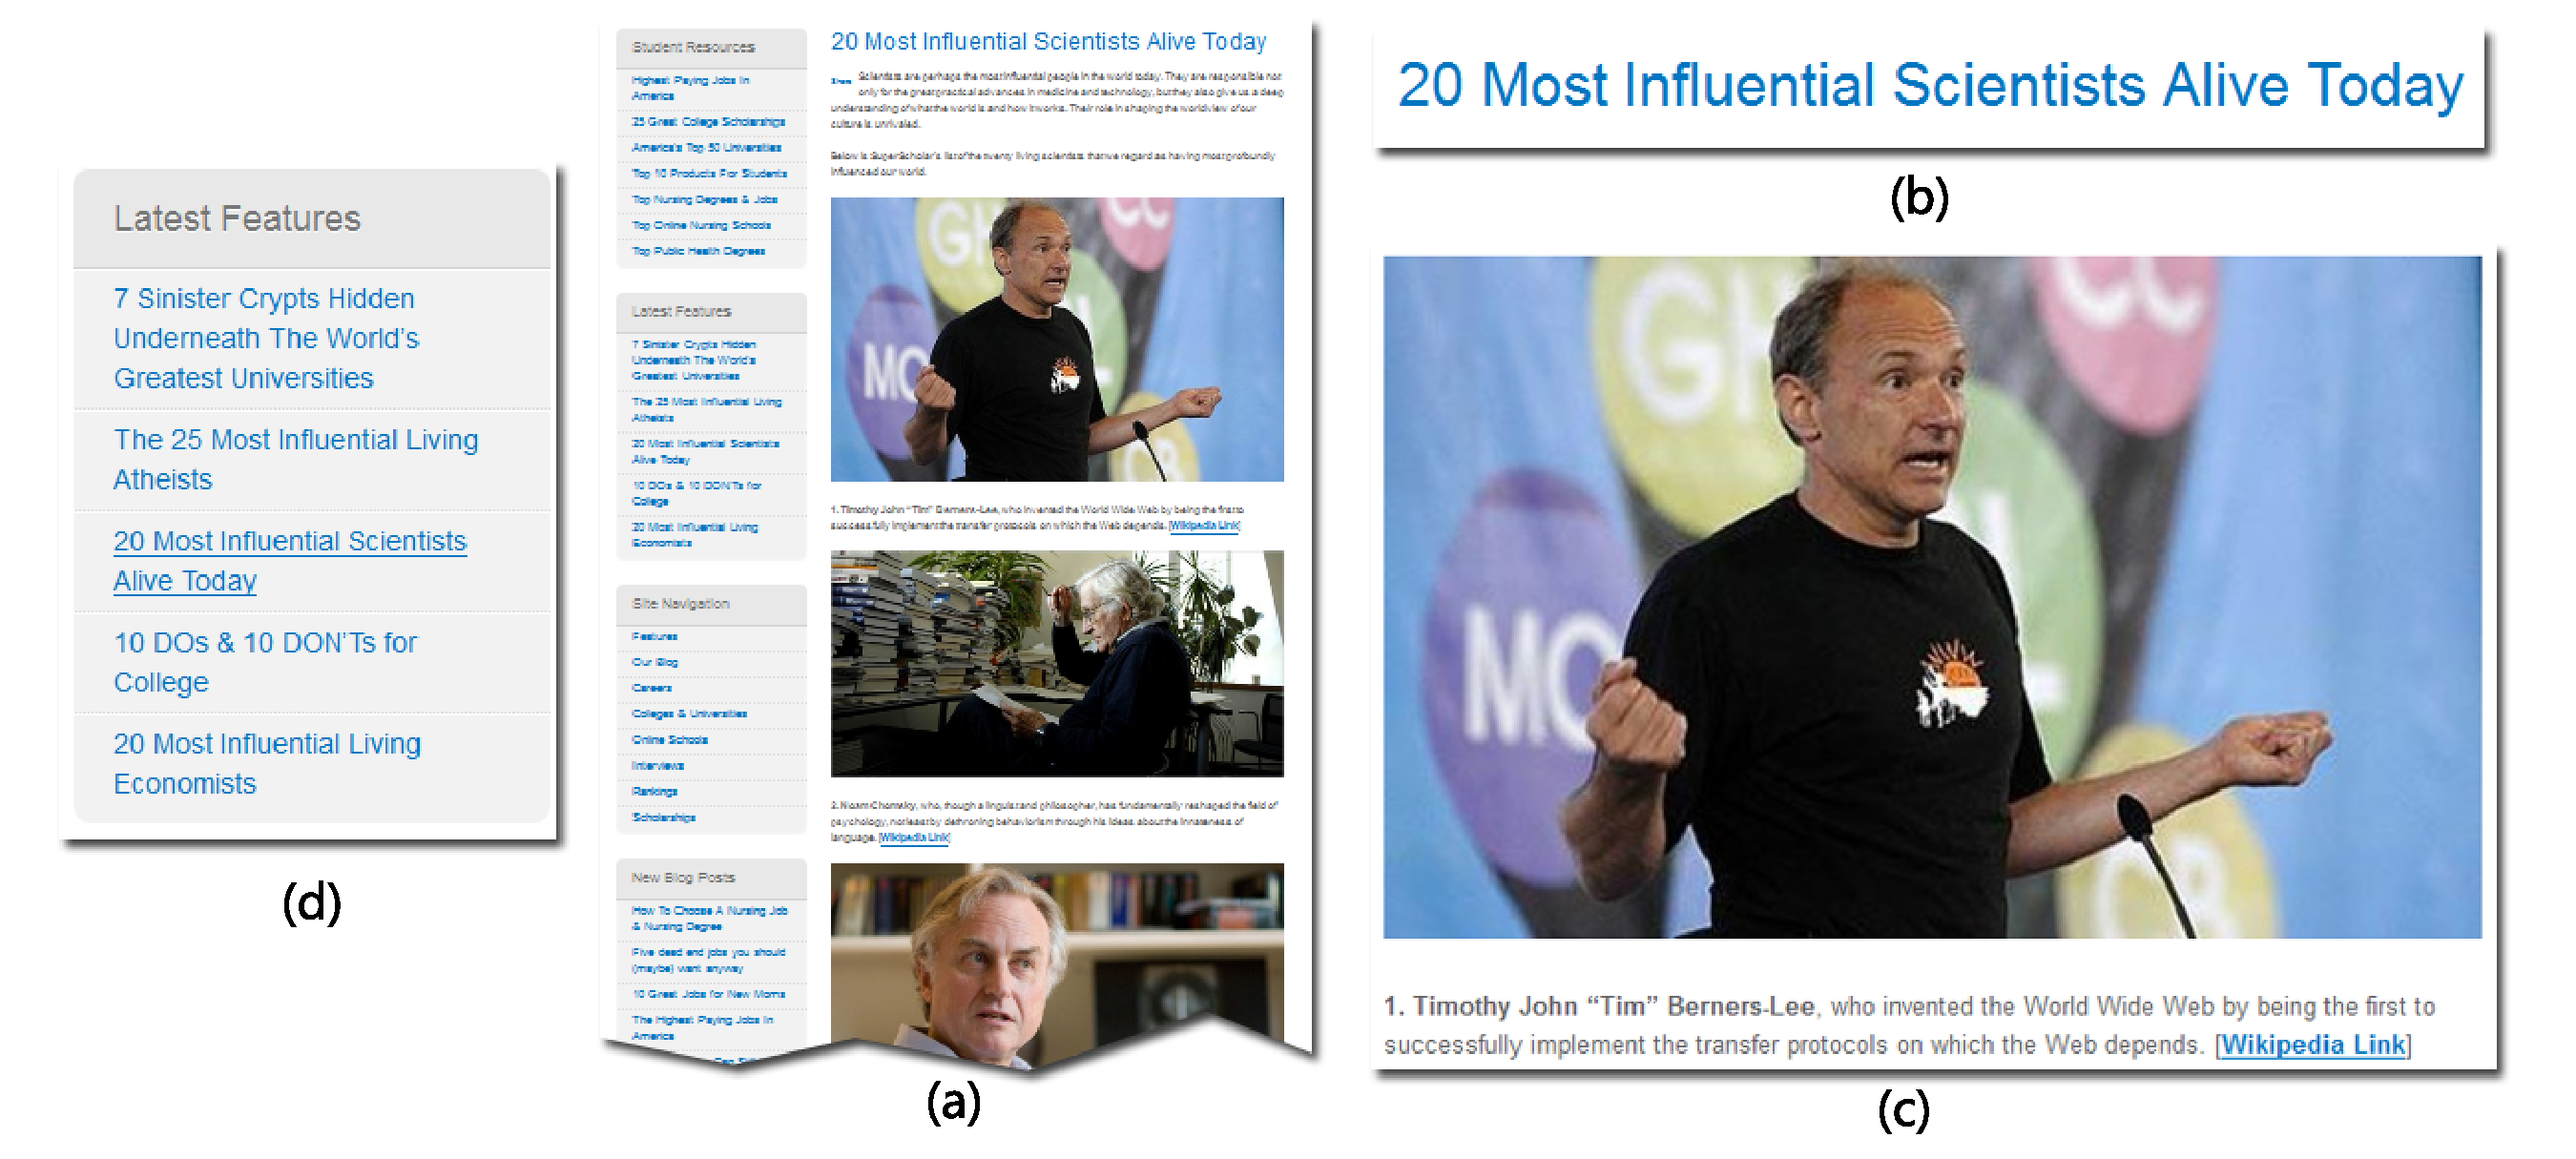
\epsfig{file=./pic/page5_detail.eps,width=1.8\columnwidth}
	\caption{A {\em top-k page} snapshot}
	\label{fig:snapshotOfWebPage}
\end{figure*}

According to the definition of the problem, our goal is the top-$k$ list,
or in other words, the data record list of the page.
Thus, we need to find $k$ Data Records to form the List.

From the analysis and statistics of many example pages, 
we assume the following property is true:

\begin{newproperty}\label{prop-1}
The corresponding data record components in one data record list share the same tag path.
\end{newproperty}

Fig?? shows a top-$k$ page as an example to explain this property.

Therefore, we would like to pick up a set of DOM tree node lists which satisfy two conditions:

1. the count of the node in the list equals the target number $k$.

2. the tree nodes share the same tag path.

In our approach, this process is called ``candidate check''. 
We consider this set as a candidate set, while each node list is a candedate list.
According to the \ref{prop-1}, some of the candidate lists may contain data record components,
and we can trace those lists to get the data record list.
Given the fact that the parent nodes of a candidate list also satisfy the conditions of a candidate list, 
as long as those parent nodes are different from each other.
Furthermore, the parent node list covers a larger visual area 
and is closer to the data record list that we want.
Therefore, 
we put the parents of a candidate node list together to form a new list and replace the original one.
We keep doing this
until some nodes in the candidate list has the same parent.
which breaks the first condition of a candidate list.
In our approach, this process is called ``growing up'', 
and the lists after the process are grown-up candidiate lists.

If there are multiple grown-up candidate lists, we have to pick one as the final data record list.
According to the definition of VRA, we infer the following property.

\begin{newproperty}\label{prop-2}
A candidate list that occupies a larger VRA has a higher importance in a page.
\end{newproperty}

Therefore, we choose the grown-up candidate list with largest VRA as our result.


Having got the data record list, 
the general goal of our problem has fulfilled.
But in our further study,
some data record components,such as pictures and descriptions are useless and should be filtered,
while the names of list items is more valuable, which are encapuslated in data record titles
Thus, we offer a optional function to extract the titles from the data record list.
Since we do not specify the topic of pages we handle
and data records have a variety of forms and styles,
it is difficult to come up with a general rule that is fit for all cases.
On the one hand, if the rule is too strict, 
it will filter some useful information in data record titles and reduce the recall of total approach.
On the other hand, 
some noise information like comments and descriptions will still remain in the result.
However, we still try to make a tride-off between the two sides, and find several several properties:
\begin{newproperty}\label{prop-3}
In most cases, a data record title should occupy only one paragraph(line) in a data record.
\end{newproperty}

\begin{newproperty}\label{prop-4}
In most cases, a data record title should be neither too long nor too short.
\end{newproperty}

\begin{newproperty}\label{prop-5}
A data record title should be relatively shorter than the description and comment text in the same data record.
\end{newproperty}

\begin{newproperty}\label{prop-6}
In most cases,a data record title should be placed before other text content in the same data record.
\end{newproperty}

 
Based on those properties, 
we build several rules which can effectively filter most noise information,
and won't do much harm to the outcome meanwhile.


At last, we also offer several optimizations, which can considerablely improve the result of the basic algorithm.
Although, the original algorithm can basicly satisfy our demand, 
we can still see the possiblity to enhance the performance.
From the study of plenty of example pages, we sum up three main kind of ``tricky'' cases that do not work on our basic algorithm:

Case 1(interleaving problem):  
For aesthetic reasons, a data record list may have a ``interleaving pattern'', which is best described in fig??.
In the basic algorithm, this kind of list may be treated as two $k/2$ lists and cannot pass the ``candidate check'' process.

Case 2($k+1$ problem):
Some page contains a ``fake'' data record, which express the list head or the conclusion of the data record list.
But the ``fake'' one has the same style and components as the real data records.
Thus the basic algorithm may put them together to form a $k+1$ list, 
which cannot pass the ``candidate check'' process.

Case 3:
Some page may has some other lists which also contain $k$ items.
Those lists may be lists of comments or advertisements 
which may be irrelavent to the page's main topic, 
but will probably comfuse our basic algorithm.

Our optimizations are aimed to handle those cases respectively, 
and result of these optimizations shows a significant growth in the precision and recall.
{\bf should I discuss the three optimizations here?}


%The section is organized as following. 
%First we will explain the basic algorithm based on tag path statistics and VRA ranking.
%The second part will discuss the methods used to handle some special cases and optimize the outcome.

In the following several subsection, we will discuss the basic algorithm, title extraction and optimizations in detail.
Also, we would like to introduce some examples to demostrate those algorithms.

\subsection{Basic Algorithm}

The Basic Algorithm of our approach is based on Property \ref{prop-1}.
{\bf to be continued...}

As shown in the Figure ??, it can be divided into 
four steps: 
{\em Preprocession}, 
{\em Candidate Selecting}, 
{\em Candidate Growing}, 
and {\em Data Record List Finding}. 
We discuss these four parts in detail below. 
In order to demostrate the algorithm more clearly, 
we would like to introduce a top-$k$ page as an example,
the snapshot of which is shown in fig??.


In {\em Preprocessing}, 
we will first turn the input web page into a DOM Tree.
In our experiment we adopt a open source HTML parser (Winista HtmlParser??) for web page parsing.

After we get the DOM Tree structure of the page, 
some normalization will be done.
In a DOM Tree, some nodes, 
such as $<head>$ and $<remark>$,
are not useful for our analysis, 
so we just filter them.
%such as filtering head node and all remark nodes

Then the process will calculate the VRA score of every tag node through the Procedure VRACal, 
which is defined as following.

\begin{algorithm}[htbp]
\caption{VRACal(aNode)}
\begin{algorithmic}[1]\label{algo:vracal}
\STATE{visualScore = 0}
\IF {aNode is a tag node}
	\FORALL{child of aNode}
	   \STATE{visualScore = VRACal(child)}
	\ENDFOR
\ELSIF{aNode is a text node}		
	\STATE{visualScore = aNode.textLength $\times$ 
			FontSize(aNode) $\times$ 
			FontSize(aNode)}
	\RETURN visualScore
\ENDIF
\end{algorithmic}
\end{algorithm}

Subprocedure FontSize(node) supplies the relative font size of 
the node based on Default style sheet for HTML4 at
\url{http://www.w3.org/TR/CSS21/sample.html}. 

We also need to go through all the DOM Tree nodes to figure out 
the frequency of all Tag Paths, defined as Procedure CountTagPath.

\begin{algorithm}[htbp]
\caption{CountTagPath(aNode, tagPathTable)}
\begin{algorithmic}[1]\label{algo:counttagpath}
	\STATE{aTagPath = GetTagPath(aNode)}
	\IF{tagPathTable contains aTagPath}
		\STATE{add aNode into tagPathTable[aTagPath]}
%		\STATE{(tagPathTable[aTagPath] as nodeList).add(aNode)}
	\ELSE	
		\STATE{let aNodeList be a new empty nodelist}
		\STATE{add (aTagPath, aNodeList) into tagPathTable}
		\STATE{add aNode into tagPathTable[aTagPath]}
%		\STATE{(tagPathTable[aTagPath] as nodeList).add(aNode)}
	\ENDIF
	\IF{(aNode is a tag node)}
		\FORALL{child of aNode}
			\STATE{GetTagPath(child,tagPathTable)}
		\ENDFOR
	\ENDIF
	\RETURN 
\end{algorithmic}
\end{algorithm}

SubProcedure {\tt GetTagPath(node)} gives the string representation 
of the node's Tag Path. The argument tagPathTable is called Tag Path Table, 
the keys of the table are Tag Paths,
and the values of table are the corresponding node lists
The VRA scores and Tag Path Table(the argument tagPathTable) will 
be stored and used in later algorithm parts.


In {\em Candidate Selecting}, 
the goal is to get the candidate set.
From the Tag Path Table, we can get a set of node lists, 
which are organized by tag paths already.
For each node list in this origin set, we adopt ``candidate check'' process,  
to decide whether to put the list in the candidate set.
Recall the \ref{prop-1} and the two conditions of a candidate list, 
we develop the following rule for ``candidate check'' process.

\begin{newrule}\label{rule-1}
If the count of the current nodelist equals to the target number $k$, 
then add it to the candidate set.
\end{newrule}

The whole step can be described as Procedure CandidateSelect.

\begin{algorithm}[htbp]
\caption{CandidateSelect(tagPathTable)}
\begin{algorithmic}[1]\label{algo:candiselect}
	\STATE{let candiSet be a new set of node list}
	\FORALL{nodeList in tagPathTable}
		\IF{nodeList contains $k$ nodes}		
			\STATE{add nodeList into candiSet}
		\ENDIF
	\ENDFOR		
	\RETURN candiSet
\end{algorithmic}
\end{algorithm}



The next step is {\em Candidate Growing}.
For each node list in this origin set, 
we adopt ``growing up'' process, 
to get the grown-up candidate lists.
This process is defined as Procedure GrowUp.

\begin{algorithm}[htbp]
\caption{GrowUp(nodeList)}
\begin{algorithmic}[1]\label{algo:growup}
	\STATE{let parentList be a new node list}
	\WHILE{TRUE}
		\FORALL{node in nodeList}
			\STATE{let parentNode be the node's parent}		
			\IF{!(parentList contains parentNode)}
				\STATE{add parentNode into parentList}						
			\ENDIF	
		\ENDFOR
		\IF{parentList.count==nodeList.count}		
			\STATE{nodeList = parentList}			
			\STATE{let parentList be a new node list}			
		\ELSE
			\STATE{break}
		\ENDIF
	\ENDWHILE	
	\RETURN nodeList
\end{algorithmic}
\end{algorithm}


We would like to maintain a new set to hold all the grown-up candidate lists.

It is worth mentioning that, 
two different candidate lists may grow up into the same grown-up list,
as shown in fig??.
In that case, we just keep one grown-up list in the new set.

In the last step, we need to find out the final result, 
the data record list.
If there is one or zero list in the new candidate set, 
the problem is simple because we can just return the node list as our answer 
or return``fail'' to indicate such a list do not exist.
Otherwise, we need to choose one from the new candidate set.
Base on \ref{prop-2}, we apply the following rule for making the choice.

\begin{newrule}\label{rule-2}
Choose the candidate node list with largest VRA as the data record list.
\end{newrule}

Since we have got the VRA of all tag nodes, we can easily get the VRA of a cadidate node list 
by simply summing up VRAs of all nodes.

\subsection{Title Extraction}

Assuming that we have got a data record (represented by the root node of a DOM tree), 
our goal of this subsection is to get the data record title.

Based on \ref{prop-6}, we build a framework of the algorithm, 
described by Procedure TitleExtract.

\begin{algorithm}[htbp]
\caption{TitleExtract(node)}
\begin{algorithmic}[1]\label{algo:title}
	\STATE{let title be a empty string}
	\WHILE{TRUE}
		\STATE{temp = NextString(node)}		
		\IF{temp != "" AND RulePass(title,temp)}		
			\STATE{title = title + temp}
		\ELSE
			\STATE{break}
		\ENDIF
	\ENDWHILE	
	\RETURN nodeList
\end{algorithmic}
\end{algorithm}

SubProcedure NextString returns the plain text in each text node
in postorder traverse. It will return an empty string if we have go through the tree.

SubProcedure RulePass is an alternative procedure 
which decides whether or not string $temp$ to be a part of $title$.
As a result, the mechanism of RulePass is the key to our algorithm 
determining the result title of the data record.

For example, if we simply let RulePass return TRUE for all cases,
we will get all the plain text extracted. 
For the data record showed in Figure ??,
all the plain text is listed in Figure ??. 

From \ref{prop-3}, we develop \ref{rule-3}.

\begin{newrule}\label{rule-3}
If there is a linebreak detected between $title$ and $temp$, return FALSE, otherwise reture TRUE.
\end{newrule}

In order to detect a linebreak in DOM tree structures, 
we summed up all the tag types that may cause a linebreak,
shown in Figure ??.
We name them as linebreak tags.

Assume that we can get the text node $n1$ of string $temp$
and its previous text node $n0$
(the string of which should be included in $title$ already),
the following three cases indicate a linebreak inbetween:

Case 1:
A linebreak tag is an ancient of $n1$ but not $n0$.
Shown in Figure?? (a)

Case 2:
A linebreak tag is an ancient of $n0$ but not $n1$.
Shown in Figure?? (b)

Case 3:
A linebreak tag occurs between $n0$ and $n1$.
Shown in Figure?? (c)

In order to detect all the three cases,
we keep the preorder and postorder of the tree 
and check the nodes between $n0$ and $n1$ 
($n0$ should be before $n1$ in both preorder and postorder,
since they are both leaves).
once we find one of them are a linebreak tag, 
we detect the linebreak and stop the algorithm.

From \ref{prop-4}, we develop \ref{rule-4}.

\begin{newrule}\label{rule-4}
If the length of $title$ plus $temp$ is over the threshold length $MaxLength$, return FALSE.
\end{newrule}

The parameter $MaxLength$ is decided by the specific topic of the data record.
In our experiment, we just make it 100.

From \ref{prop-4}, we develop \ref{rule-4}.

\begin{newrule}\label{rule-4}
If the length of $temp$ is  longer than $t$ times that of $title$, return FALSE.
\end{newrule}

Similarly, the parameter $t$ is decided by the specific topic of the data record.
which is 1 in our experiment.

We can apply any of the three rules above to gain different effect and result.
Also, we can combine the three rules in RulePass together 
which has a better experimental outcome.


\subsection{Optimizations}

We would like to dicuss the three optimizations we propose 
respectively in this subsection.

\subsubsection*{Interleaving Problem}

Just like the exmple shown in Figure??,
the data record list has two styles respectively 
for even and odd rows.
This fact make the odd rows get a tag path different from that of the even rows,
and
In the basic algorithm, 
the list may be treated as two $k/2$ lists 
and cannot pass the ``candidate check'' process.

Then our solution tries to check all the $k/2$ list pairs 
to see whether the two lists are interleaving.
If so,
we can merge them into one list and put them into the candidate set.
We adopt a simple method to detect two lists' interleaving
which is defined in Procedure IsInterleaving.

\begin{algorithm}[htbp]
\caption{IsInterleaving(list1,list2)}
\begin{algorithmic}[1]\label{algo:interleave}

	\IF{list2[0] < list1[0] in postorder}
		\IF{list2[0] < list1[0] in preorder}
			\STATE{swap list1 and list2}
		\ELSE
			\RETURN FALSE	
		\ENDIF		
	\ENDIF
	\STATE{i = 1}
	\WHILE{i is smaller than the count of list1}
		\IF{list2[i] < list1[0] in postorder OR list2[i] < list1[i] in preorder}
			\RETURN FALSE	
		\ENDIF		
		\STATE{i = i + 1}
	\ENDWHILE	
	\RETURN TRUE
\end{algorithmic}
\end{algorithm}

In order to make it brief, 
we do not mention some safety check in the pesudo code.

If the total number of list items($k$) are odd, this method still work after a little adjustment.
For example, we should turn to the pairs of one $k/2$ list and one $k/2+1$ list.

This method also fit the cases that the data record list contains arbitrary $p$ styles.
We just need to check all the combinations of $p$ lists that contain $k/p$ nodes.
But there are very few cases that have more than two styles in the list, 
we just omit them and only handle the cases that contain two styles.

\subsubsection*{$k+1$ problem}
Figure ?? shows a typical example to describe this problem:
after 5 data records about... , 
the page adds an additional conclusion part at last
which forms a ``fake'' data record.
Since it has the same tag path as the data records,
our basic algorithm cannot distinguish it from the $k$ ``real'' ones,
so the algorithm will put them together to form a $k+1$ list.
Also, some pages will add a list head in front of the real list, 
which may become a ``fake'' data record as well.

This situation is quite common in top-$k$ pages.
Thus, we would like to give these $k+1$ lists ``a second chance'',
using the following rule to enhance \ref{rule-1}

\begin{newrule}\label{rule-1-2}
If the count of the current nodelist equals to the target number $k+1$ , 
then delete one item of the list
and add the left to the candidate set.
\end{newrule}

There are a few ways to ``kick out'' the ``fake'' data record from a $k+1$.
For example, we can compare the subtree of each node and kick the most unique one.
Or we can look into the content of each node to find some cues 
which infer a conclusion or a list head.

Also, there is a similar case called $k-1$ problem:
one of the data records has a different style from others,
for example, the first or last data record is often highlighted (Figure??),
so we can only get a ``k-1'' list.
Of course, we could add all the $k-1$ lists into the candidate set.
But the problem how to find the ``lost'' data record is still pending.
Thus, we only handle the ''k+1`` problem in our experiment.

\subsubsection*{Tag Path Filtering}
Although, the methods discussed above can solve the problems very well,
it also brings some side effect.
Since we also take all $k+1$ lists and $k/2$ lists into consideration,
the possibility that we choose a incorrect record list will increase.
Thus, we should ``shrink'' our candidate set by filtering some candidate lists.

In order to know what kind of tag can never be contained in a tag path of a data record,
we select 100 top-$k$ pages as learning examples.
We define Set $TOTAL(attr)$ as the collection 
of the words found in the attribute $attr$ of all the tags of the learning examples.
Similarly, Set $CORRECT(attr)$ contains the words
found in the attribute $attr$ of all the ancient tag nodes of data records of the learning examples.
And we can define $GREY(attr)$ by the equation $GREY(attr)=TOTAL(attr)-CORRECT(attr)$.
{\bf zzx: ee this two definitions are not brief, do you have a better statement?}
First,
we get two word sets, after the analysis of all the pages:
$GREY(ID)$,
$GREY(CLASS)$.
We choose the attribute ID and CLASS because they are most popular attributes of tags.
Then we sort the words in $GREY(ID)$ and $GREY(CLASS)$ by their frequency,
and choose the top 10 most frequent words in each set 
to form the final blacklist, which is shown in table??.
With the blacklist we get, we can filter node lists by the following rule.

\begin{newrule}\label{rule-filter}
If any word is contained in the tag path of the node list, the list should be filtered.
\end{newrule}

Actually, this method is quite effective 
that we can get rid of most noise list from comment and advertisment area
after filtering.

